\documentclass[11pt,a4paper]{article}
\usepackage[utf8]{inputenc}
\usepackage[english]{babel}
\usepackage[margin=0.8in]{geometry}
\usepackage{amsmath}
\usepackage{amsfonts}
\usepackage{amssymb}
\usepackage{graphicx}
\usepackage{float}
\author{Tom Stappaerts - Bachelor Informatica \and Jeroen Sanders - Bachelor Informatica}
\title{Computer Networks \& Network Simulation \\ \begin{small} Prof: Danny Hughes\end{small}}
\begin{document}
\maketitle
\newpage 

\section{Exercise 1}

\subsection{Question 1}
\begin{figure}[h!]
 \centering
 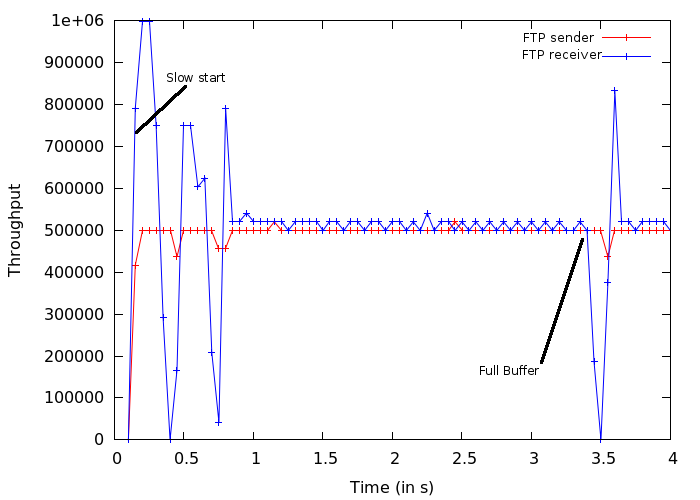
\includegraphics[width = 0.8\linewidth]{./output-ex1-part1-2-5.png}
 % output-ex1-part1-2-5.png: 700x500 pixel, 72dpi, 24.69x17.64 cm, bb=0 0 700 500
 \caption{Throughput: bandwidth limitation and download connection}
 \label{fig:Q1}
\end{figure}
In figure \ref{fig:Q1} we plotted the throughput the sender and receiver of the FTP application. We see that after a 'slow start' the connection stabilises on 5 Mbps.
This is higher than what the connection of the modem can handle. Therefore we see a drop in throughput at the sender after the buffer fills up (3.5 sec). The download is limited by the strained connection between node 3 and 4.

\subsection{Question 2}
\begin{figure}[h!]
 \centering
 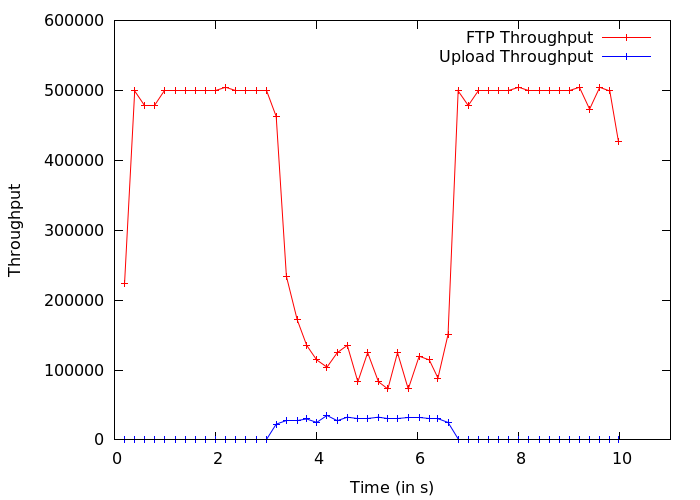
\includegraphics[width = 0.8\linewidth]{./output-ex1-part-2-1-7.png}
 % output-ex1-part-2-1-7.png: 700x500 pixel, 72dpi, 24.69x17.64 cm, bb=0 0 700 500
  \caption{Throughput: bandwidth limitation, download and upload connection}
 \label{fig:Q2}
\end{figure}
The FTP application uses all the available bandwidth. As soon as the CBR pplication starts it clogs up the network. It's packages are bigger than the tcp acknowledgement packages and it takes quite a while to upload them through the constrained upload link. That's why we see a big drop in the graph. The buffer to the FTP downloader still has some packets so they continue to arrive, as you can see in figure \ref{fig:Q1}.

\subsection{Question 3}
A reserved amount of upload bandwidth for each application would prevent cannibalisation of the connection. A certain throughput would be guaranteed for both applications. Initially the FTP application would behave just like in question 1. When the CBR application starts, it's bandwidth will decrease because the CBR application has it's own guaranteed bandwidth. It is expected that the CBR application would perform better. The exact amount of dropped packets for the CBR application would depend on the exact amount of available bandwidth.

\subsection{Question 4}
\begin{figure}[h!]
 \centering
 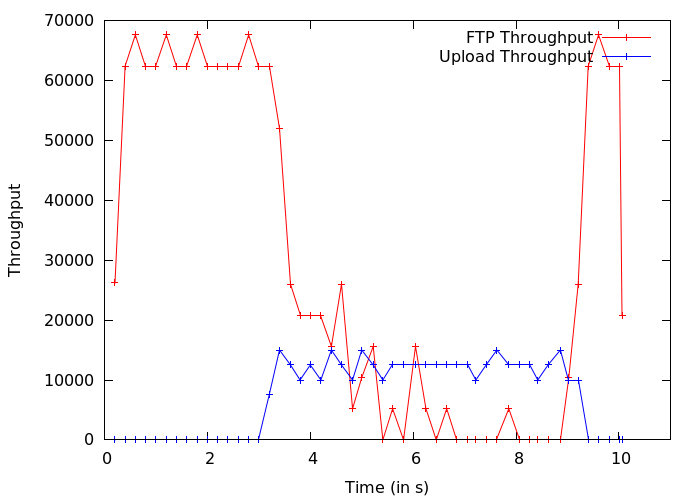
\includegraphics[width = 0.8\linewidth]{./ex1-part-4-1-7.png}
 % ex1-part-4-1-7.png: 700x500 pixel, 72dpi, 24.69x17.64 cm, bb=0 0 700 500
 \caption{Throughput: bandwidth limitation, download and upload: even more restricted}
 \label{fig:Q4}
\end{figure}
If the bandwidth is even more constrained, the saturation of the network is even higher. It's worse because it takes longer for the buffers to clear. The throughput of the FTP application crashes to zero, and cannot increase while the buffers are full with data of the CBR application. 

\subsection{Question 5}
\begin{figure}[h!]
 \centering
 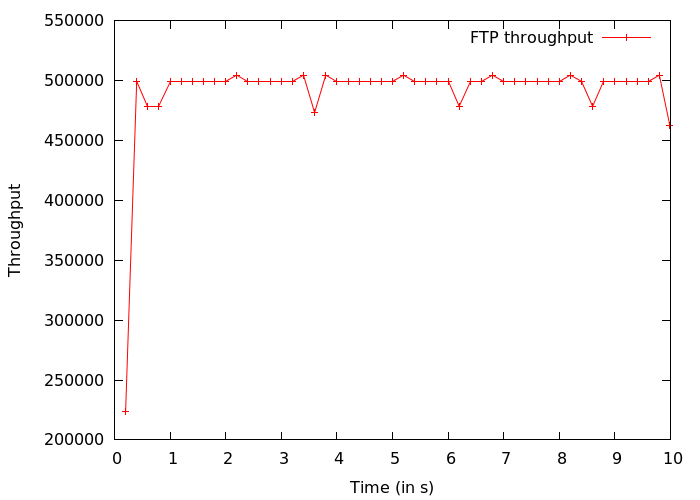
\includegraphics[width = 0.8\linewidth]{./output-ex1-part5.png}
 % output-ex1-part5.png: 700x500 pixel, 72dpi, 24.69x17.64 cm, bb=0 0 700 500
 \caption{Throughput: upload rate at 30 000}
 \label{fig:Q5}
\end{figure}
When the CBR upload connection is fixed to a rate of 30 kbps the FTP connection is not hindered by it.
To prevent hosts from interfering with each other, you could implement some sort of load balancing between hosts. In practice this would result in a (weighted) round-robin queue instead of a FIFO queue.  

\end{document}
